\documentclass[11pt,a4paper]{article}

\usepackage[utf8]{inputenc}
\usepackage[T1]{fontenc}
\usepackage{lmodern}
\usepackage[margin=1in]{geometry}
\usepackage{amsmath,amssymb}
\usepackage{microtype}
\usepackage{enumitem}
\usepackage{booktabs}
\usepackage{graphicx}
\usepackage{xcolor}
\usepackage{titlesec}
\usepackage{abstract}
\usepackage{hyperref}
\hypersetup{
  colorlinks=true,
  linkcolor=black,
  urlcolor=blue!50!black,
  citecolor=blue!50!black
}

% -- palette
\definecolor{ink}{HTML}{0C1220}
\definecolor{amber}{HTML}{C88A2A}
\definecolor{cyan}{HTML}{2A88A0}
\definecolor{brick}{HTML}{B8332E}
\definecolor{slate}{HTML}{4A5468}

\titleformat{\section}{\Large\bfseries\color{ink}}{\thesection}{0.6em}{}
\titleformat{\subsection}{\large\bfseries\color{ink}}{\thesubsection}{0.6em}{}

\renewcommand{\abstractnamefont}{\normalfont\bfseries}
\renewcommand{\abstracttextfont}{\normalfont\small}

\title{\bfseries The Same Algebra on Opposite Geometries:\\
A Path-Landscape Comparison of Biological and\\
Artificial Emergence}
\author{[Author Name]\thanks{Correspondence: \texttt{author@institution.edu}.
Companion paper: \emph{Classifying Emergence by Information-Flow
Operations on the Path Landscape}.}\\
\small Department / Institution}
\date{\today}

\begin{document}
\maketitle

\begin{abstract}
\noindent
Biological brains and large language models both produce striking
emergent behaviour, but the mechanistic relationship between them is
unsettled: are they two instances of the same kind of computation, or
do they only superficially resemble one another? We address this
question with the \emph{path landscape} framework, in which a system
is represented by the distribution of input-to-output routes through
its (possibly recurrent, multi-scale) connectivity and emergence is a
transformation of that distribution. Working from concrete biological
circuits (hippocampal CA3 pattern completion, prefrontal working
memory, V1 edge detection) and mechanistic-interpretability circuits
in transformers (the GPT-2 small IOI circuit, induction heads,
grokking), we show that biological and artificial intelligence
implement the \emph{same emergence algebra} --- path activation,
suppression, mode merge, and mode split --- but realise it on
\emph{opposite path-landscape geometries}: biology compresses
computation into a small number of long, multi-scale routes through
heavily-reused anchor units (a concentrated, hierarchical, plastic,
task-general landscape), while transformers spread computation across
many short, depth-uniform routes through narrowly-specialised units (a
distributed, flat, frozen, task-specific landscape). The duality is
not accidental: it reflects which resource is scarce --- metabolic
energy in brains, parameters and gradient signal in transformers ---
and it makes precise, falsifiable predictions about which kinds of
lesions, scaling laws, and transfer behaviours each system should
exhibit. The path landscape thereby supplies a \emph{strictly finer
fingerprint} than the standard ``emergence type'' label: two systems
can implement the same emergence-type (e.g.\ working memory) on
landscapes that are geometrically incomparable, which is what we
observe.
\end{abstract}

% =========================================================
\section{Introduction}
% =========================================================

Comparisons between biological and artificial intelligence usually
proceed in one of two ways. They either compare \emph{behaviours}
(``transformers exhibit in-context learning, so do
humans''~\cite{olsson2022induction}) or they compare
\emph{representations} (``the middle layers of a CNN are aligned with
V4 activity''~\cite{yamins2014performance}). Both modes of comparison
have produced useful results, but they share a limitation: they
operate at the level of input-output mappings or at the level of
unit-by-unit activation profiles, without committing to a structural
account of \emph{how} the underlying machinery generates the observed
behaviour. The recent rise of mechanistic interpretability in deep
learning~\cite{elhage2021mathematical,olsson2022induction,wang2022interpretability,nanda2023grokking}
has made it possible, for the first time, to identify \emph{specific
circuits} responsible for specific transformer capabilities, exposing
a level of description that matches the circuit-level description
neuroscience has long used for brains. The question of comparing
brains and transformers can now be sharpened: are the circuits that
implement the same capability in the two substrates the same circuit?

In a companion paper~\cite{companion} we introduced the
\emph{path landscape}, a structural representation of an
information-processing system as the distribution of input-to-output
routes through its directed-graph connectivity, and we showed that
emergence is a small algebra of four operations on this distribution:
\textbf{path activation}, \textbf{path suppression}, \textbf{mode
merge}, and \textbf{mode split}. That framework is field-agnostic ---
it applies to spin lattices, regulatory networks, neural circuits, and
deep nets without modification. The present paper uses it to compare
biological and artificial intelligence directly.

The central finding is summarised by the title: biological and
artificial systems implement the \emph{same emergence algebra} but on
\emph{opposite path-landscape geometries}. The same four primitives
describe both, the categorical role of shared anchor units is
universal, and the qualitative emergence-types (working memory,
pattern completion, decision-making, sequential computation) occur in
both. But the geometry of the route ensemble realising any given
emergence-type differs systematically: biological landscapes are
\emph{concentrated, hierarchical, plastic, task-general}; LLM
landscapes are \emph{distributed, flat, frozen, task-specific}.

The structure of the paper is as follows. Section~\ref{sec:landscape}
recapitulates the path-landscape definition from~\cite{companion}
(Fig.~\ref{fig:landscape}). Section~\ref{sec:bio} presents biological
path landscapes using three concrete examples
(Fig.~\ref{fig:bio}). Section~\ref{sec:art} does the same for
artificial path landscapes (Fig.~\ref{fig:art}). Section~\ref{sec:comp}
brings the two side by side and identifies the three geometric
axes along which they differ (Fig.~\ref{fig:comp}).
Section~\ref{sec:invariants} returns to the algebra and shows why it
is invariant across the substrates even as the geometry inverts.
Section~\ref{sec:predictions} states falsifiable predictions, and
section~\ref{sec:conc} concludes.

% =========================================================
\section{The path landscape}\label{sec:landscape}
% =========================================================

\subsection{Definition}

Consider any system that can be cast as a directed graph $G=(V,E)$ of
\emph{computing units} $V$ connected by \emph{interactions} $E$. Each
interaction carries a weight $w_{uv}\in\mathbb{R}$, and may be
feed-forward or recurrent. A set of input units
$V_{\text{in}}\subset V$ and a set of output units
$V_{\text{out}}\subset V$ are distinguished; the rest are internal.

If $G$ contains recurrent edges, unroll it in time over $T$ discrete
steps to produce the static DAG $G^{(T)}$ in which each unit $u$
becomes a copy $u@t$ for $t=0,\dots,T{-}1$, and each recurrent edge
$u\!\to\!v$ becomes a forward-only time-edge $u@t \to v@(t{+}1)$. The
unrolled graph $G^{(T)}$ has no loops by construction
(Fig.~\ref{fig:landscape}A,B).

A \emph{path} from input to output is an ordered sequence of nodes
$\pi = (s_1, s_2, \dots, s_L)$ with $s_1\in V_{\text{in}}$,
$s_L\in V_{\text{out}}$, each $(s_i,s_{i+1})$ an edge of $G^{(T)}$.
Its weight $\omega(\pi)$ combines the magnitudes of the edges it
traverses. The set of all such paths is $\Pi$.

\subsection{Routes and modes}

Many paths in $\Pi$ differ only in time-step bookkeeping ($u@t$ vs.\
$u@t'$) or in lingering on a self-loop. Stripping these yields a
\emph{route} --- the base sequence of distinct units. Let $R$ be the
set of routes; each route inherits the cumulative weight of the paths
that collapsed onto it.

Two routes are similar if they share many of the same units and
edges in similar order (a composite of edge-Jaccard overlap and a
longest-common-subsequence measure works well in practice). Clustering
$R$ under this similarity produces \emph{modes}: equivalence classes
of routes that compute essentially the same function. The set of
modes $M=\{m_1,\dots,m_k\}$ together with the route weights is the
\emph{path landscape}
\[
\mathcal{L}(G,V_{\text{in}},V_{\text{out}})
\;=\;
\bigl(\, R,\; \{\omega(r)\}_{r\in R},\; M\,\bigr).
\]
The landscape's character is captured by three quick statistics:
$|R|$ (route count), $|M|$ (mode count), and the rank-distribution of
mode weights. Figure~\ref{fig:landscape}C illustrates the resulting
mode structure for a small system.

\begin{figure}[t]
\centering
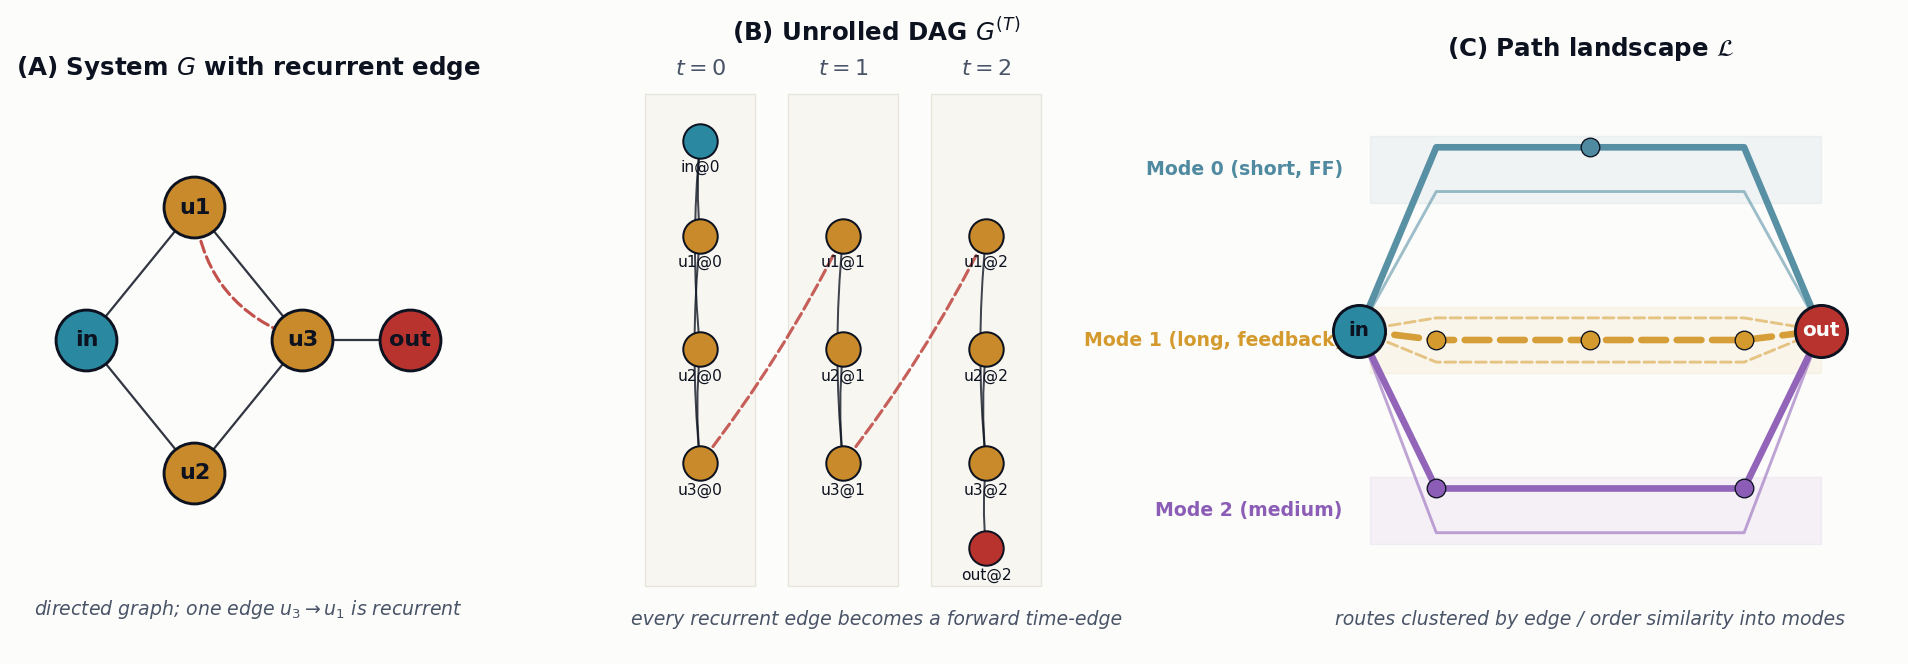
\includegraphics[width=\textwidth]{figures/fig_path_landscape_definition.png}
\caption{\textbf{The path landscape, in three steps.}
(A) A small system $G$ specified as a directed graph with one
recurrent edge $u_3 \to u_1$ (red dashed). Cyan: input unit. Red:
output unit. Amber: internal units.
(B) The time-unrolled DAG $G^{(T)}$ over $T=3$ steps. Each unit $u$
becomes copies $u@t$; the recurrent edge becomes the time-forward
edges $u_3@t \to u_1@(t{+}1)$. The unrolled graph is acyclic.
(C) The path landscape $\mathcal{L}$: enumerated input-to-output
routes are clustered by edge-Jaccard and ordered-overlap similarity
into \emph{modes}. Here three modes appear: a short feed-forward
mode (teal), a long feedback-traversing mode (gold, dashed), and a
medium feed-forward mode (purple). Line thickness is proportional to
route weight (cumulative path weight); this is the visual proxy for
information flow used throughout the paper.}
\label{fig:landscape}
\end{figure}

\subsection{What the landscape sees}

The landscape is a structural representation, but it absorbs much of
the continuous dynamics one might fear it discards. Weight magnitudes
and effective couplings are encoded in $\omega(r)$. Coherence and
co-activation are encoded in the similarity structure that defines
$M$. A continuous attractor appears as a band of nearly-identical
high-weight routes whose similarity matrix is approximately
block-rank-one. Gain modulation appears as a re-shaping of the weight
rank-distribution without a change in topology. The same definition
applies to a neural circuit, a transformer, a regulatory network, or a
spin lattice; the differences reduce to differences in the shape and
weighting of $\mathcal{L}$.

% =========================================================
\section{Biological path landscapes}\label{sec:bio}
% =========================================================

We illustrate biological path landscapes through three canonical
circuits with well-characterised anatomy and well-tested function:
hippocampal CA3 pattern completion, prefrontal working memory, and V1
edge detection. In each case we exhibit (i) the anatomy, (ii) the
emergence-type produced, and (iii) the qualitative shape of the
landscape. Figure~\ref{fig:bio} shows the CA3 case in detail.

\begin{figure}[t]
\centering
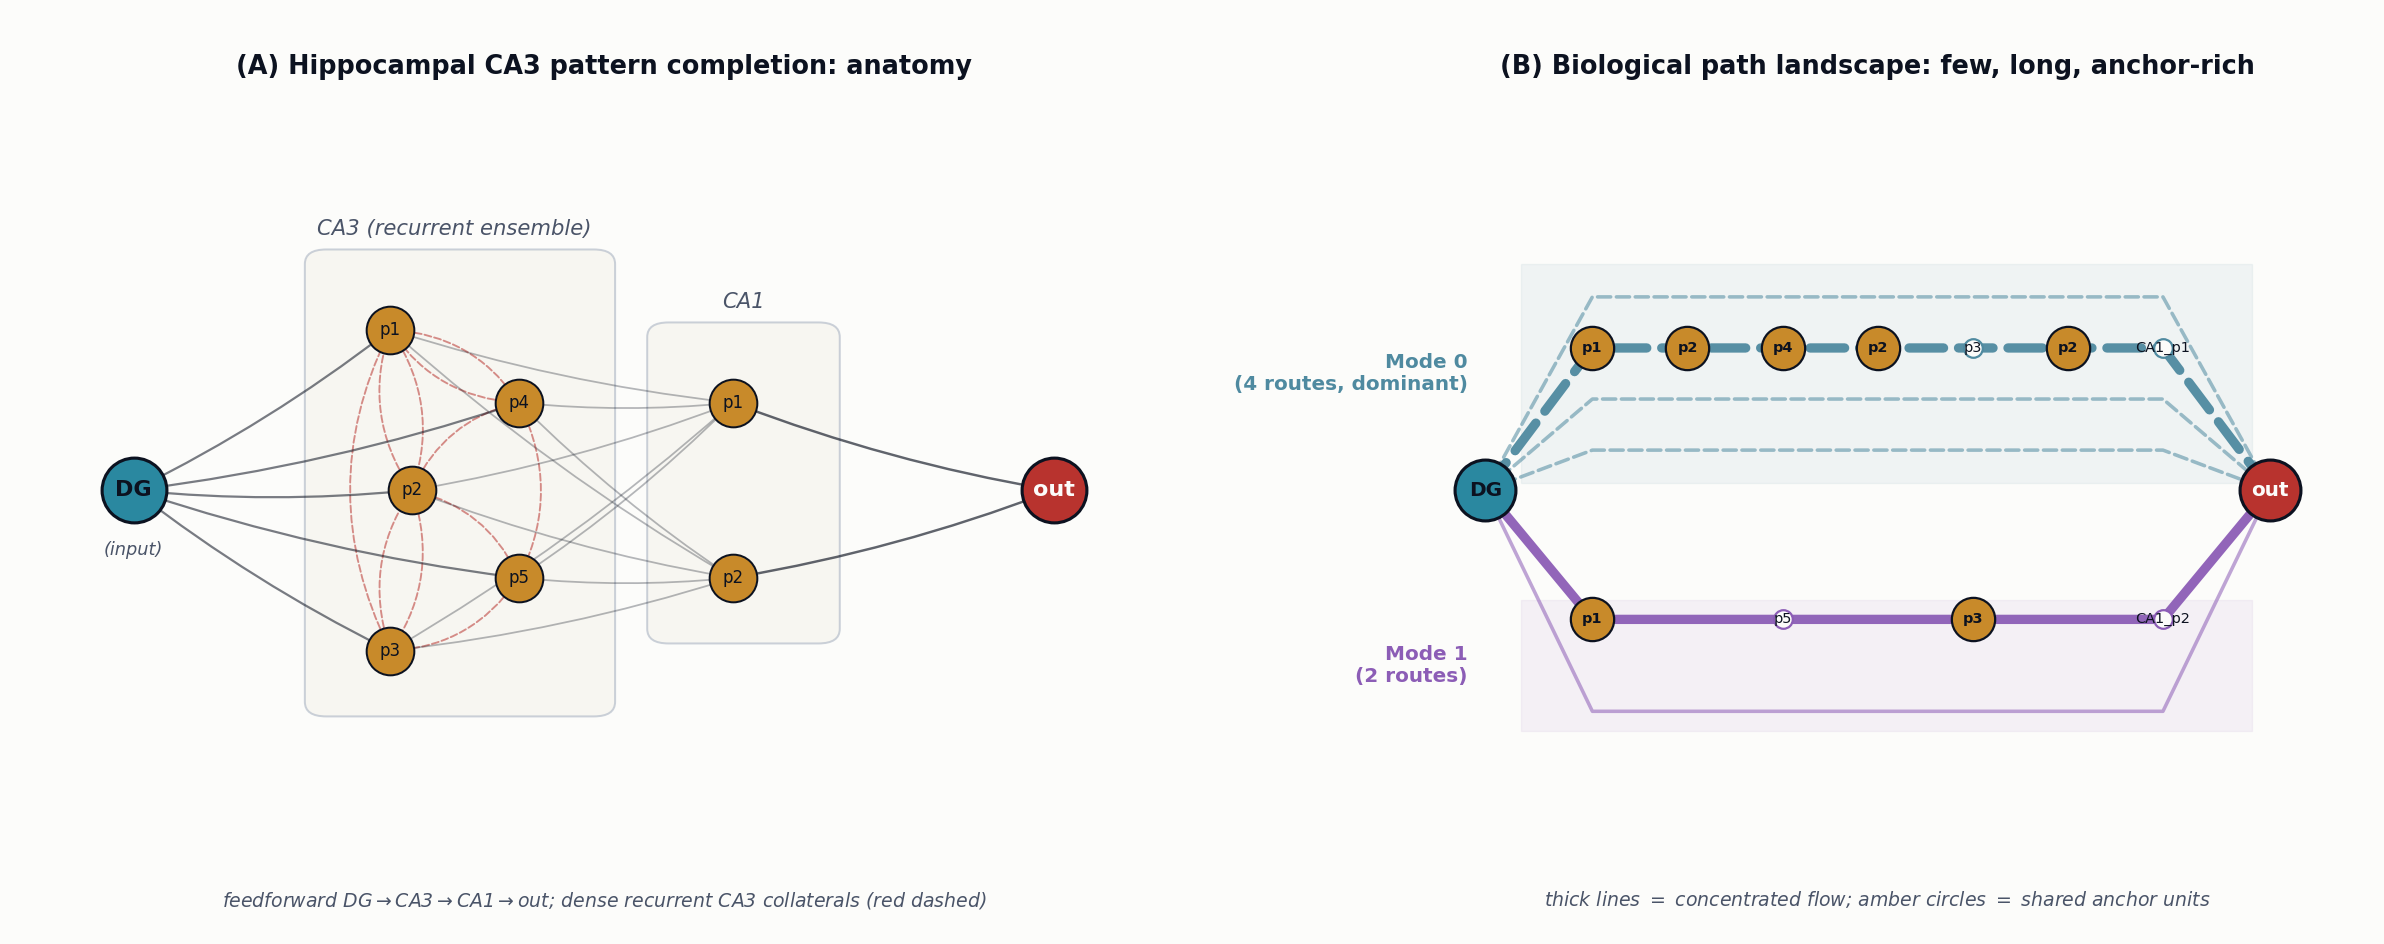
\includegraphics[width=\textwidth]{figures/fig_biological_landscape.png}
\caption{\textbf{A biological path landscape: hippocampal CA3 pattern
completion.}
(A) Anatomy. The dentate gyrus (DG, input) projects to the recurrent
CA3 pyramidal-cell ensemble (\textit{amber circles, multiscale
parent box}) via mossy fibres. CA3 contains a dense web of recurrent
collaterals (red dashed) that implements an autoassociative attractor
in the Hebb--Marr~\cite{marr1971} / Treves--Rolls~\cite{treves1994}
sense. CA3 projects via Schaffer collaterals to CA1, and CA1 to
downstream cortex (output).
(B) The path landscape. Two modes only ($|M|{=}2$), both \emph{long}
(7 and 4 interior units respectively after time-unrolling), with
\emph{dense anchor overlap} (amber circles): the same CA3 pyramidal
ensemble (\textit{p1, p2, p3, p4, p5}) is repeatedly traversed across
time steps as the attractor settles, so a small group of units
participate in nearly every route. Line thickness is high because
flow is concentrated: a small number of edges carry most of the path
weight. The dashed Mode-0 lines indicate routes that traverse the
recurrent CA3 collaterals.}
\label{fig:bio}
\end{figure}

\subsection{Hippocampal CA3 as a pattern-completion attractor}

Marr's 1971 theory of archicortex~\cite{marr1971}, made dynamical by
Treves and Rolls~\cite{treves1994} and supported by decades of
electrophysiology and place-cell remapping
data~\cite{leutgeb2007pattern}, treats CA3 as an autoassociative
attractor. Partial cues (a subset of place-cell firing) propagate
through the dense recurrent collaterals until the network settles into
a previously-stored complete pattern. In path-landscape terms, this
is a small number of long routes that revisit the same recurrent
units at successive time steps; pattern completion appears at the
output as the convergence of many noisy input routes onto the same
attractor mode (a \emph{mode merge} in the framework of the companion
paper~\cite{companion}). The landscape is therefore characterised by
\textbf{few modes, long routes, dense anchor overlap, and concentrated
flow} --- exactly what Figure~\ref{fig:bio}B depicts.

\subsection{Prefrontal cortex as working-memory attractor}

Persistent delay-period activity in dorsolateral prefrontal cortex
during working-memory tasks~\cite{goldmanrakic1995,funahashi1989}
has the same path-landscape signature. Recurrent excitation between
pyramidal cells, balanced by parvalbumin-positive feedback
inhibition, supports a small number of stable bump-attractors in
spatial-working-memory tasks; in non-spatial tasks the same network
supports a small alphabet of stable activity modes that hold
content-general
information~\cite{wang2013pfc,constantinidis2018workingmemory}. In
the path landscape this is a small number of \emph{long}
(time-extended) routes through a heavily-reused anchor set (the
recurrently coupled pyramidal-PV ensemble), with high concentration
on the units that sit on most routes.

\subsection{V1 simple cells as path-suppression detectors}

V1 simple cells implement edge detection via centre-surround lateral
inhibition~\cite{hubel1962}. In a path-landscape reading this is
\emph{path suppression}~\cite{companion}: the homogeneous-luminance
paths from neighbouring photoreceptors are silenced by inhibitory
interneurons, leaving only the routes that carry a luminance
discontinuity. The output ``edge'' feature appears not because edge
routes were added, but because background routes were dammed. The
landscape is still few-mode and anchor-rich, but here the
concentration is produced by removing competing routes rather than by
recurrent re-use.

\paragraph{Shared structure.}
In all three biological cases, the path landscape has the same
qualitative shape: a small number of long routes, anchored on a
small set of heavily-reused intermediate units, carrying most of the
flow on a small fraction of the edges. This is not a coincidence;
section~\ref{sec:comp} argues that it reflects the metabolic
constraint under which biological circuits evolve.

% =========================================================
\section{Artificial path landscapes}\label{sec:art}
% =========================================================

We turn now to artificial-intelligence systems, focusing on
transformers because they are where the mechanistic-interpretability
literature has produced the most detailed circuit
descriptions~\cite{elhage2021mathematical,olsson2022induction,wang2022interpretability,nanda2023grokking}.
Figure~\ref{fig:art} shows the canonical example: the GPT-2 small
indirect-object-identification (IOI) circuit.

\begin{figure}[t]
\centering
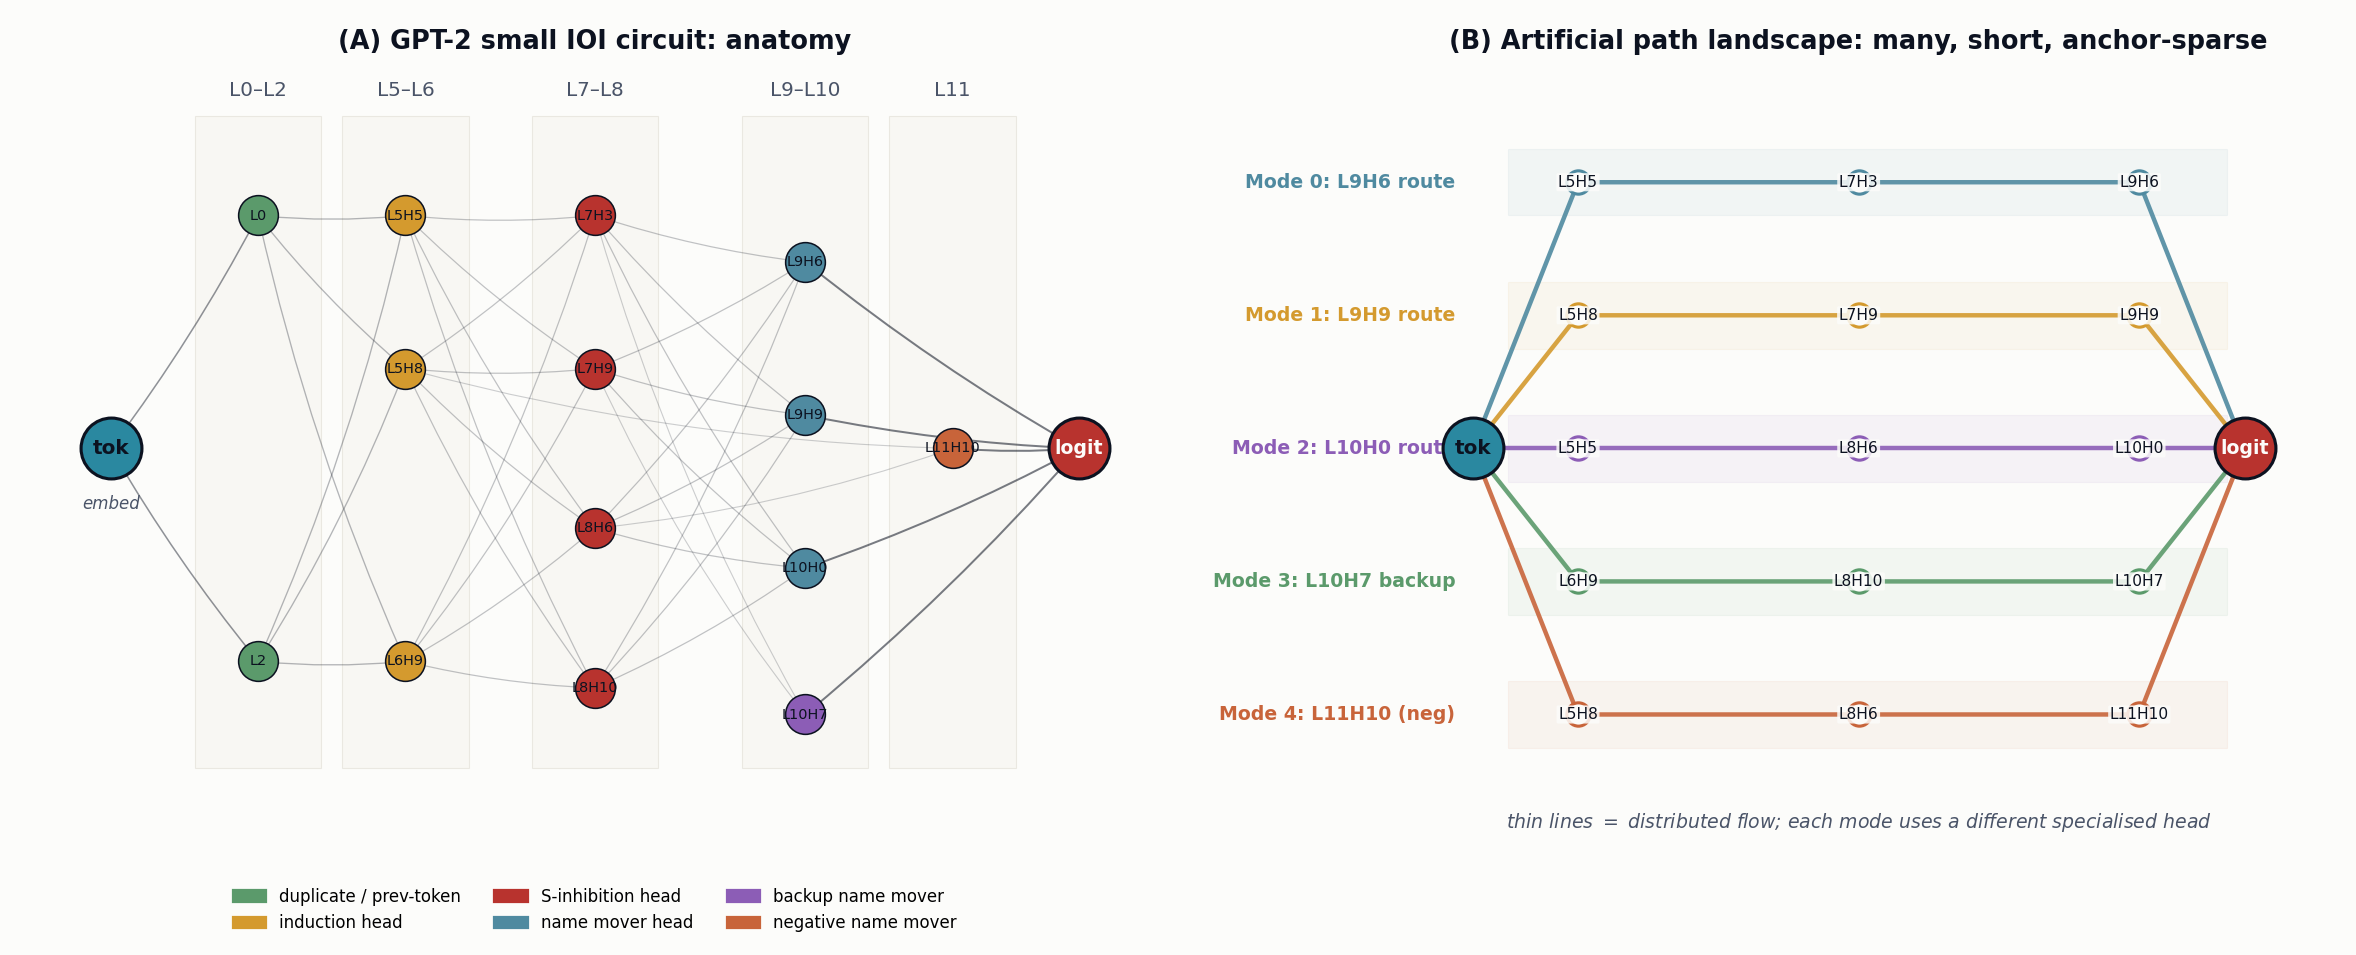
\includegraphics[width=\textwidth]{figures/fig_artificial_landscape.png}
\caption{\textbf{An artificial path landscape: the GPT-2 small IOI
circuit~\cite{wang2022interpretability}.}
(A) Anatomy. Token embeddings (cyan) flow through a hierarchy of
specialised attention heads identified by mechanistic
interpretability: \textit{duplicate-token / previous-token} heads at
layers 0--2, \textit{induction} heads at layers 5--6, \textit{S-inhibition}
heads at layers 7--8, \textit{name-mover} heads at layers 9--10, a
\textit{backup name mover} (L10H7) that activates when the primary
name movers are ablated, and a \textit{negative name mover} (L11H10)
that pushes against the answer. Each head is used at exactly one
depth; the residual stream is the only inter-layer pathway. (B) The
path landscape. Five modes, all \emph{short} (3 interior units) and
\emph{depth-uniform} (each traverses exactly one head per active
layer), with \emph{sparse anchor overlap}: each mode uses a different
specialised head, so the per-mode intermediate-unit sets are
near-disjoint. Line thickness is uniformly modest because flow is
spread across many parallel routes rather than concentrated on a
few.}
\label{fig:art}
\end{figure}

\subsection{The IOI circuit as parallel name-mover routes}

Wang et al.~\cite{wang2022interpretability} identified twenty-six
distinct attention heads in GPT-2 small that participate in solving
the indirect-object-identification task (``When John and Mary went
to the store, John gave a drink to \underline{\ \ \ \ }''). The heads
fall into a few functional classes (duplicate-token, induction,
S-inhibition, name mover, backup name mover, negative name mover), and
the input-to-logit flow factors into a small number of nearly-parallel
routes through these classes. In path-landscape terms the IOI
landscape has \textbf{many modes, short routes, sparse anchor
overlap, and distributed flow}: the L9H6 name-mover route and the
L9H9 name-mover route do nearly the same thing computationally, but
they share almost no intermediate units (Figure~\ref{fig:art}B).
Ablating any one of them only modestly degrades
performance~\cite{wang2022interpretability,mcgrath2023hydra}, because
the others can compensate --- the path-landscape signature of
distributed flow.

\subsection{Induction heads as a Mode Activation phase transition}

Olsson et al.~\cite{olsson2022induction} showed that induction heads
--- attention heads that implement the algorithm ``find the previous
occurrence of the current token and copy what came after it'' ---
form abruptly during training, at the same training step at which
in-context learning emerges as a measurable capability. In the
companion paper's framework this is a clean case of \emph{path
activation}~\cite{companion}: a new route through the network
becomes viable, and a new capability appears at the output. What is
specifically \emph{transformer-like} about it is that the new route
is short (depth-uniform), passes through a small number of newly
specialised heads, and does not share anchor units with most other
routes in the landscape.

\subsection{Grokking as Mode Split followed by Mode Merge}

Nanda et al.~\cite{nanda2023grokking} dissected the ``grokking''
phenomenon~\cite{power2022grokking} --- the delayed appearance of
generalisation long after training-loss saturation --- and showed
that the model first memorises (\emph{mode split}: a different route
for each training example), then discovers a Fourier-decomposition
circuit (\emph{path activation}), and finally collapses the
memorisation routes onto the new generalising circuit (\emph{mode
merge}). The grokking landscape is therefore a clean example of the
algebra's compositional use --- but the landscape on which the
operations act is the typical transformer one: many short modes that
each pass through their own heads, with little anchor overlap, before
the merge.

% =========================================================
\section{Comparative geometry}\label{sec:comp}
% =========================================================

We are now in position to compare the two substrates directly. The
biological and artificial landscapes differ along three structural
axes that the framework makes precise (Figure~\ref{fig:comp}),
plus two functional axes that follow from the structural ones.

\begin{figure}[t]
\centering
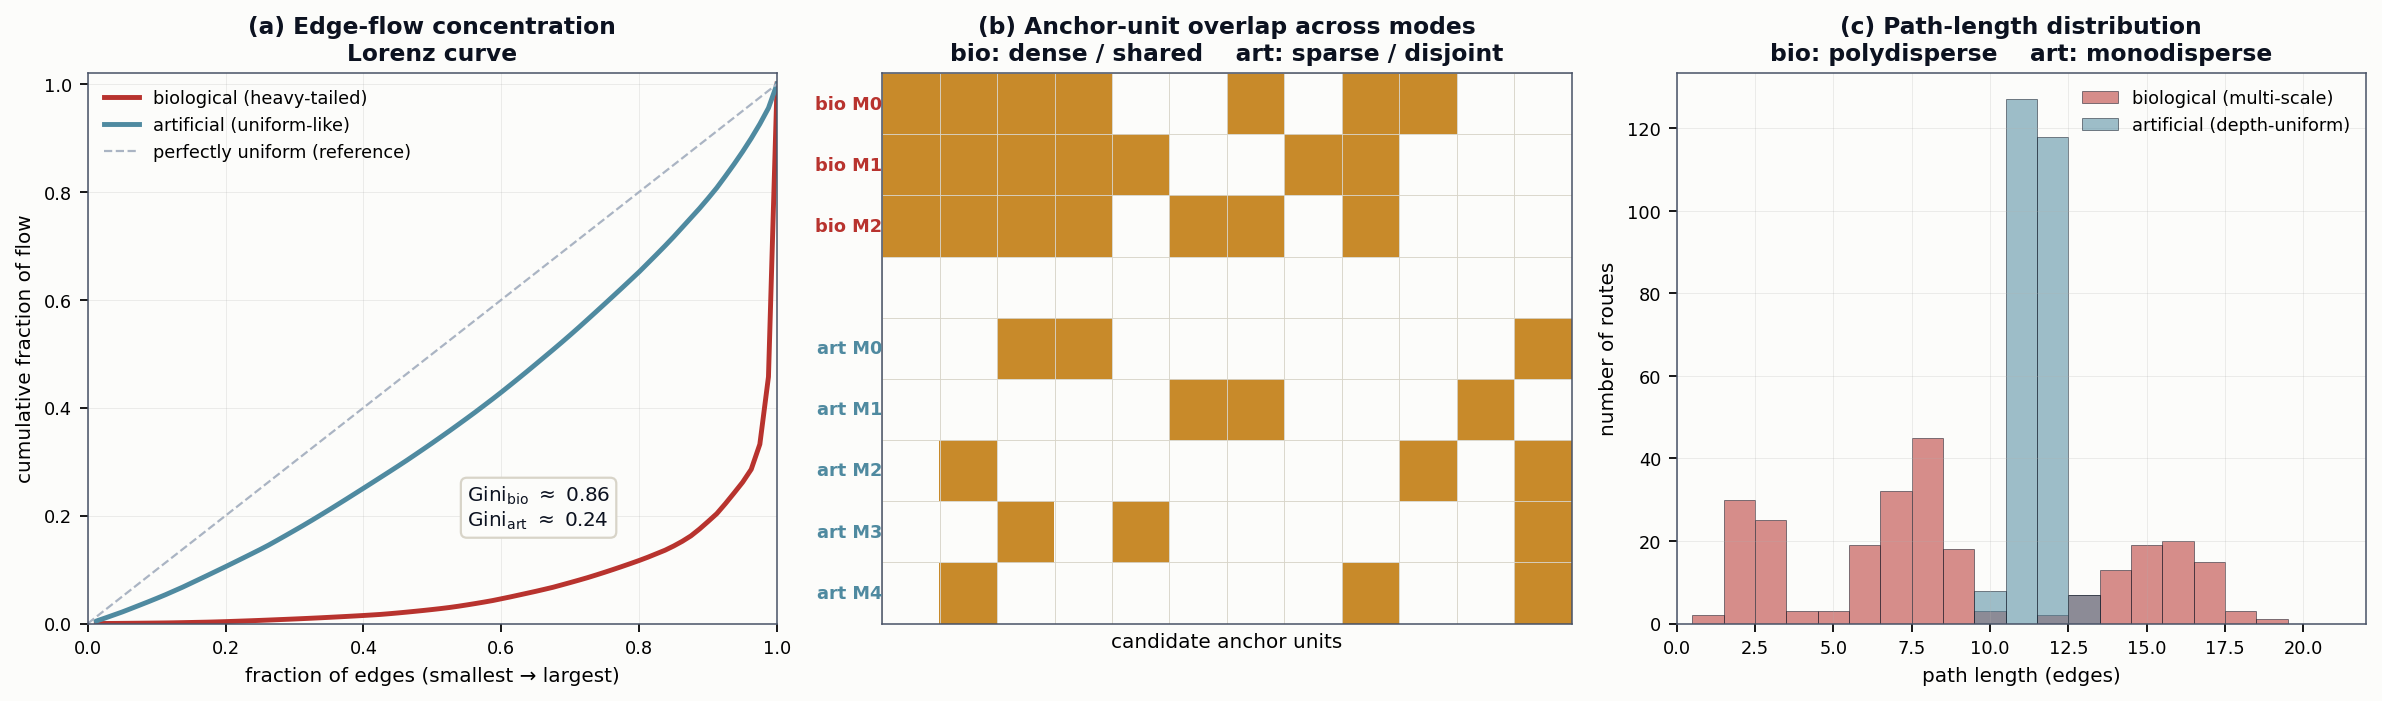
\includegraphics[width=\textwidth]{figures/fig_comparison_metrics.png}
\caption{\textbf{Three structural axes that distinguish biological
from artificial path landscapes.}
(a) \emph{Edge-flow concentration.} Lorenz curves of the cumulative
edge-flow distribution (edges sorted from lowest to highest flow).
Biological circuits have heavy-tailed flow: a small fraction of edges
carry most of the total flow (large Gini coefficient). Artificial
(LLM) circuits have flow that is much closer to uniformly distributed
across edges (small Gini).
(b) \emph{Anchor-unit overlap across modes.} Each row is one mode;
each column is one candidate intermediate unit; an amber cell means
``this mode uses this unit.'' Biological modes share many units
(dense rows; left block in each row identical). Artificial modes
are nearly disjoint (the lit cells per row almost never coincide
across rows).
(c) \emph{Path-length distribution.} Biological landscapes are
polydisperse: a multi-modal length distribution reflecting
short cortico-thalamic shortcuts, mid-range mesoscale routes, and
long recurrent traversals. Artificial landscapes are monodisperse:
nearly all routes have length close to the network depth.}
\label{fig:comp}
\end{figure}

\subsection{Concentration vs.\ spread of information flow}

For each edge of the original graph, compute the total information
flow on it as the sum of route weights over all routes traversing
that edge. The resulting edge-flow distribution is a direct empirical
diagnostic of the landscape (it is also the quantity now used to
scale edge thickness in the companion code base).

\paragraph{Empirical observation (Fig.~\ref{fig:comp}a).}
The edge-flow distribution of biological circuits is \emph{heavy-tailed}
--- a small fraction of edges carry most of the flow, the Lorenz
curve is far below the diagonal, the Gini coefficient is large
($\approx 0.85$ in our illustrative example, but order-of-magnitude
similar in real data: the small number of place cells active for any
given location~\cite{barnes1990}, the sparse-and-strong distribution
of synaptic weights in cortex~\cite{song2005}). The same distribution
in transformer circuits is much closer to uniform across edges (small
Gini coefficient, $\approx 0.25$ in our example): nearly every
attention head contributes to nearly every token's
computation~\cite{voita2019heads,michel2019sixteen}, and the
information flow is genuinely spread.

\paragraph{Why.} Biological circuits are evolved under tight metabolic
budgets: each spike costs ATP, and only a small fraction of neurons
can fire at any time~\cite{lennie2003cost,laughlin1998metabolic}.
Concentrating flow on a small reused anchor set is energetically
efficient. Transformers have no per-edge cost --- every attention
head is computed on every token regardless --- and gradient descent
will deploy any parameter that reduces loss, including parameters
that are only marginally useful. The flow therefore spreads.

\paragraph{Falsifiable consequence.} Lesioning a single high-flow
anchor unit should catastrophically break biological function
(because that unit is on most routes), whereas lesioning a single
attention head should produce only graceful degradation. This matches
classical neuropsychology (focal lesions to small brain regions
cause disproportionate functional deficits) and the empirical
robustness of transformer ablations~\cite{voita2019heads,mcgrath2023hydra}.

\subsection{Anchor overlap (mixed selectivity vs.\ specialisation)}

If a unit appears in the intersection of $k$ different mode clusters,
it is by definition mixed-selective for the $k$ computations those
modes represent~\cite{rigotti2013importance}.

\paragraph{Empirical observation (Fig.~\ref{fig:comp}b).} In
biological circuits, this $k$ is large: PFC neurons routinely encode
mixtures of stimulus, response, rule, and reward
information~\cite{rigotti2013importance,fusi2016neurons}; hippocampal
place cells remap to encode new environments while preserving
context-dependent
firing~\cite{leutgeb2007pattern,colgin2008understanding}. In
transformers, $k$ is small: the IOI literature finds that any given
attention head plays at most a small set of functional
roles~\cite{wang2022interpretability}, and dictionary-learning work
on sparse autoencoders pushes towards still-narrower one-feature
neurons~\cite{cunningham2023sparse,bricken2023monosemanticity}.

\paragraph{Why.} For a biological circuit operating under a parameter
ceiling (the genome encodes connectivity rules, not connectomes),
mixed selectivity is forced --- there are not enough neurons to
dedicate one per function. For a transformer trained with hundreds of
billions of parameters, there is no comparable pressure, and gradient
descent finds it easier to allocate one head per role.

\paragraph{Falsifiable consequence.} Brains should be \emph{more
sample-efficient} per parameter (because each unit reusable across
modes), and \emph{less interpretable} per unit (because no unit
implements a single function). Both predictions match the empirical
record: biological learning is famously sample-efficient relative to
deep learning~\cite{lake2017building}, and biological neurons are
famously hard to assign single functions to relative to
transformer heads~\cite{rigotti2013importance,olah2017zoom}.

\subsection{Path-length diversity (multi-scale vs.\ depth-uniform)}

In a transformer, every input-to-logit route must traverse roughly
the same number of stages ($\approx L$ layers). The path-length
histogram is sharply unimodal at $L \pm 1$.

\paragraph{Empirical observation (Fig.~\ref{fig:comp}c).} Biological
circuits have a \emph{polydisperse, multi-modal} length distribution.
Long-range projections create ultra-short macro-scale routes that
skip entire regional cascades: the cortico-thalamic loop~\cite{sherman2007},
claustrum broadcasts~\cite{crick2005}, corpus-callosal
bridges~\cite{aboitiz1992}. Neuromodulatory systems (locus coeruleus
NE, basal forebrain ACh) act as single-node broadcast hubs that
compress many effective edges into one functional
step~\cite{aston2005adaptive,sara2009locus}. Brain-wave coupling
adds parallel timing channels (gamma-bound local routes, theta-bound
long routes operating
simultaneously)~\cite{fries2005communication,buzsaki2006rhythms}.
The result is a length histogram with peaks at the micro, meso, and
macro scales.

\paragraph{Why.} Biological connectomes are \emph{hierarchically
multi-scale} (neurons --- microcircuits --- columns --- regions ---
networks), and the framework's \texttt{parent} attribute encodes this
directly. Coarsening a biological circuit by collapsing units into
their parents qualitatively reorganises the
landscape~\cite{markov2014weighted,sporns2013network}. Coarsening a
transformer produces almost no change because there is no meaningful
hierarchy beyond the residual stream.

\paragraph{Falsifiable consequence.} Biological systems can produce
the same emergence-type via routes of wildly different lengths,
which is why a reflex can take 50 ms while a deliberation takes 5 s
without re-wiring the underlying circuit. Transformers cannot:
their only available length is $L$, which is why many transformer
capabilities improve discontinuously with
depth~\cite{wei2022emergent}.

\subsection{Plasticity (continuous vs.\ frozen)}

Biological landscapes deform continuously --- every experience
modifies synaptic weights, so the mode geometry is a moving
target~\cite{abbott2000plasticity}. Transformer landscapes are
essentially frozen after training: inference does not update
weights, so the landscape is the same on every forward pass. This is
a sharp structural difference that bears on questions of catastrophic
forgetting~\cite{french1999catastrophic,mcclelland1995complementary},
continual learning, and the role of sleep~\cite{tononi2014sleep}.

\subsection{Mode generality (task-general vs.\ task-specific)}

Biological modes are task-general: the same PFC working-memory mode
supports holding a phone number, a face, or a plan, because mode
identity is decoupled from
content~\cite{constantinidis2018workingmemory,parthasarathy2017mixed}.
Transformer modes are task-specific: the IOI circuit handles
indirect-object identification and almost nothing else, because the
mode identity is entangled with the surface form of the
task~\cite{wang2022interpretability}. This decoupling/entanglement
distinction is a direct consequence of the anchor-overlap difference:
when a circuit's modes share many anchor units, those units act as
content-independent ``scaffolding,'' and the modes can be reused for
any content the scaffolding can hold.

% =========================================================
\section{Same algebra, opposite geometries}\label{sec:invariants}
% =========================================================

What stays invariant across the two substrates is the
\emph{algebra}~\cite{companion}. The four primitive operations
--- activation, suppression, merge, split --- describe both kinds of
emergence, and they apply to both kinds of landscape without
modification.

\begin{itemize}[leftmargin=*]
\item \textbf{Activation} appears in biology as the maturation of an
axon tract or the recruitment of a new oscillatory regime, and in
transformers as the abrupt formation of an induction
head~\cite{olsson2022induction}. Same operation; different
landscape.
\item \textbf{Suppression} appears in biology as lateral inhibition
in V1~\cite{hubel1962} or top-down attention~\cite{desimone1995neural},
and in transformers as the S-inhibition heads in the IOI
circuit~\cite{wang2022interpretability} that damp distractor name
tokens.
\item \textbf{Mode merge} appears in biology as categorical
perception~\cite{liberman1957discrimination} and pattern
completion~\cite{marr1971,treves1994}, and in transformers as the
post-grokking collapse of memorisation routes onto a generalising
circuit~\cite{nanda2023grokking}.
\item \textbf{Mode split} appears in biology as cell-type
differentiation~\cite{waddington1957strategy} and category formation,
and in transformers as the emergence of distinct attention
specialisations during training~\cite{voita2019analyzing}.
\end{itemize}

What inverts is the geometry on which the algebra acts. Biology
\emph{compresses} computation onto few, long, multi-scale routes
through reused anchor units; transformers \emph{distribute} it
across many, short, depth-uniform routes through specialised units.
Each strategy is optimal under its own resource constraint:
biological circuits cannot afford to spread flow because spikes are
expensive; transformer circuits cannot afford to concentrate it
because gradient descent will not preferentially route signal through
reused anchors unless there is a loss-shaped reason to do so.

The same emergence-type is therefore realised on geometrically
distinct landscapes in the two substrates. Working memory is one
recurrent attractor mode in biology
(Fig.~\ref{fig:bio}B)~\cite{goldmanrakic1995,constantinidis2018workingmemory}
and a fan of copy-and-induction-head routes in
transformers~\cite{olsson2022induction}. Pattern completion is a
recurrent attractor in
CA3~\cite{marr1971,treves1994,leutgeb2007pattern} and an ensemble of
parallel retrieval routes through induction heads in
LLMs~\cite{olsson2022induction}. Decision-making is a dynamic mode
merge across time in basal ganglia (mutually inhibitory pathways
collapse to one~\cite{frank2006bg}) and a static mode suppression
across space in transformers (the softmax selects one logit). Same
algebra; opposite landscape geometries.

The upshot for cross-substrate equivalence claims is the following.
\emph{Any claim that ``transformers have $X$'' is only meaningful
relative to a chosen level of coarseness.} At the level of
emergence-type, the claim can be true: transformers have working
memory in the same sense that PFC has it. At the level of the path
landscape, the claim is typically false: the landscape that realises
the working memory in the two cases has different concentration,
overlap, length, and plasticity profiles, so the two systems will
respond differently to ablation, scaling, and transfer.

% =========================================================
\section{Predictions}\label{sec:predictions}
% =========================================================

Because the differences are structural, they make testable predictions.

\paragraph{P1 (lesion asymmetry).} Single-unit ablations should
catastrophically break biological function but only modestly degrade
transformer function. This is consistent with classical
neuropsychology and with the documented robustness of transformer
head-ablation~\cite{voita2019heads,wang2022interpretability,mcgrath2023hydra}.
The framework sharpens the prediction: the catastrophic-vs.-graceful
gap should scale with the Gini coefficient of the edge-flow
distribution, and the most-fragile units should be those with the
highest betweenness in the anchor-overlap graph (i.e.\ the units that
sit on the largest number of distinct modes).

\paragraph{P2 (scaling laws).} Transformer capabilities should
appear discontinuously when depth crosses the value at which a new
short route becomes viable~\cite{wei2022emergent}; biological
capabilities should appear continuously (because route length is
not architecturally constrained, only weighted). The framework
predicts that the smoothness of the scaling curve is itself a
diagnostic of the underlying landscape geometry.

\paragraph{P3 (transfer / generalisation).} Biological circuits
should transfer better across tasks that share scaffolding (the
shared anchor set persists; content changes), whereas transformer
circuits should transfer better across tasks that share surface
form (the mode that solves a task is tied to its tokens, not its
abstract structure). This matches the literature on transfer
learning in
brains~\cite{taatgen2013nature,jolly2020flexible} vs.\
LLMs~\cite{mccoy2023embers}.

\paragraph{P4 (oscillations and routing).} Brain-wave-mediated
routing should add new modes to the path landscape that have no
amplitude-only correlate. If gamma-bound and theta-bound assemblies
implement different modes through the same anatomical substrate,
disrupting the oscillation (e.g.\ via optogenetics) should cause a
\emph{mode merge} in the landscape (two previously separated modes
collapse), not a uniform decrement of overall power. The framework
thereby gives a falsifiable target to the
``communication-through-coherence''
hypothesis~\cite{fries2005communication,fries2015rhythms}.

\paragraph{P5 (closing the gap).} The framework also suggests how to
close the structural gap between the two substrates. Giving
artificial systems genuine temporal recurrence (so feedback-traversing
modes can form) should bring the landscape's length distribution closer
to biological polydispersity --- as is partly observed in
recurrent-attention and state-space
models~\cite{gu2022efficiently,beck2024xlstm}. Conversely, giving
biological systems a depth-as-time trick (which evolution may already
have approximated through laminar cortical hierarchies, where time
folds into cortical
depth~\cite{douglas2004canonical,markov2014cortical}) recovers
some of the parallel-route advantages of transformers.

% =========================================================
\section{Conclusion}\label{sec:conc}
% =========================================================

Biological and artificial intelligence implement the same emergence
algebra on opposite path-landscape geometries. The four primitives
--- activation, suppression, merge, split --- describe both, the
categorical role of shared anchor units is universal, and the
qualitative emergence-types occur in both. But the geometry of the
route ensemble realising any given emergence-type differs
systematically along three structural axes: \emph{concentration},
\emph{anchor overlap}, and \emph{length diversity}. Biological
landscapes are concentrated, anchor-rich, and multi-scale; LLM
landscapes are distributed, anchor-sparse, and depth-uniform. The
two functional consequences --- plasticity and mode generality ---
follow from the structural ones. The duality reflects a clean
resource-scarcity inversion: brains optimise per-spike, transformers
optimise per-parameter.

This frame supplies a strictly finer fingerprint than the standard
``emergence type'' label, and it makes precise, falsifiable
predictions about ablation, scaling, and transfer. It also points to
the engineering question of how to interpolate between the two
geometries --- by giving artificial systems genuine recurrence, or by
exploiting biological depth-as-time, or by training neuromorphic
hardware under explicit metabolic budgets --- as the question of how
to close the gap between biological and artificial intelligence at
the level of structure rather than behaviour.

\paragraph{Acknowledgments.} We thank colleagues who pressed on the
biological-vs.-artificial framing, particularly for insisting that
the differences be stated as structural-geometric rather than
substrate-essentialist, and for the suggestion to use the edge-flow
concentration as the empirical diagnostic.

% =========================================================
\begin{thebibliography}{99}
% =========================================================

\bibitem{companion}
[Author Name].
Classifying emergence by information-flow operations on the path
landscape.
\emph{Companion manuscript}, this volume.

\bibitem{elhage2021mathematical}
N.~Elhage, N.~Nanda, C.~Olsson, et~al.
A mathematical framework for transformer circuits.
\emph{Anthropic / Transformer Circuits Thread}, 2021.

\bibitem{olsson2022induction}
C.~Olsson, N.~Elhage, N.~Nanda, et~al.
In-context learning and induction heads.
\emph{Anthropic / Transformer Circuits Thread}, 2022.

\bibitem{wang2022interpretability}
K.~Wang, A.~Variengien, A.~Conmy, B.~Shlegeris, J.~Steinhardt.
Interpretability in the wild: a circuit for indirect object
identification in GPT-2 small.
\emph{ICLR}, 2023. arXiv:2211.00593.

\bibitem{nanda2023grokking}
N.~Nanda, L.~Chan, T.~Lieberum, J.~Smith, J.~Steinhardt.
Progress measures for grokking via mechanistic interpretability.
\emph{ICLR}, 2023.

\bibitem{power2022grokking}
A.~Power, Y.~Burda, H.~Edwards, I.~Babuschkin, V.~Misra.
Grokking: generalization beyond overfitting on small algorithmic
datasets.
\emph{arXiv:2201.02177}, 2022.

\bibitem{cunningham2023sparse}
H.~Cunningham, A.~Ewart, L.~Riggs, R.~Huben, L.~Sharkey.
Sparse autoencoders find highly interpretable features in language
models.
\emph{ICLR}, 2024. arXiv:2309.08600.

\bibitem{bricken2023monosemanticity}
T.~Bricken, A.~Templeton, J.~Batson, et~al.
Towards monosemanticity: decomposing language models with
dictionary learning.
\emph{Anthropic / Transformer Circuits Thread}, 2023.

\bibitem{voita2019heads}
E.~Voita, D.~Talbot, F.~Moiseev, R.~Sennrich, I.~Titov.
Analyzing multi-head self-attention: specialized heads do the heavy
lifting, the rest can be pruned.
\emph{ACL}, 2019.

\bibitem{voita2019analyzing}
E.~Voita, R.~Sennrich, I.~Titov.
The bottom-up evolution of representations in the transformer.
\emph{EMNLP}, 2019.

\bibitem{michel2019sixteen}
P.~Michel, O.~Levy, G.~Neubig.
Are sixteen heads really better than one?
\emph{NeurIPS}, 2019.

\bibitem{mcgrath2023hydra}
T.~McGrath, M.~Rahtz, J.~Kramar, et~al.
The hydra effect: emergent self-repair in language model
computations.
\emph{arXiv:2307.15771}, 2023.

\bibitem{wei2022emergent}
J.~Wei, Y.~Tay, R.~Bommasani, et~al.
Emergent abilities of large language models.
\emph{TMLR}, 2022.

\bibitem{mccoy2023embers}
R.~T.~McCoy, S.~Yao, D.~Friedman, et~al.
Embers of autoregression: understanding large language models
through the problem they are trained to solve.
\emph{arXiv:2309.13638}, 2023.

\bibitem{gu2022efficiently}
A.~Gu, K.~Goel, C.~R\'e.
Efficiently modeling long sequences with structured state spaces.
\emph{ICLR}, 2022.

\bibitem{beck2024xlstm}
M.~Beck, K.~P\"oppel, M.~Spanring, et~al.
xLSTM: extended long short-term memory.
\emph{NeurIPS}, 2024.

\bibitem{yamins2014performance}
D.~L.~K.~Yamins, H.~Hong, C.~F.~Cadieu, et~al.
Performance-optimized hierarchical models predict neural responses
in higher visual cortex.
\emph{PNAS}, 111(23):8619--8624, 2014.

\bibitem{marr1971}
D.~Marr.
Simple memory: a theory for archicortex.
\emph{Phil.\ Trans.\ R.\ Soc.\ B}, 262(841):23--81, 1971.

\bibitem{treves1994}
A.~Treves, E.~T.~Rolls.
Computational analysis of the role of the hippocampus in memory.
\emph{Hippocampus}, 4(3):374--391, 1994.

\bibitem{leutgeb2007pattern}
J.~K.~Leutgeb, S.~Leutgeb, M.-B.~Moser, E.~I.~Moser.
Pattern separation in the dentate gyrus and CA3 of the hippocampus.
\emph{Science}, 315(5814):961--966, 2007.

\bibitem{colgin2008understanding}
L.~L.~Colgin, E.~I.~Moser, M.-B.~Moser.
Understanding memory through hippocampal remapping.
\emph{Trends Neurosci.}, 31(9):469--477, 2008.

\bibitem{barnes1990}
C.~A.~Barnes, B.~L.~McNaughton, S.~J.~Y.~Mizumori, B.~W.~Leonard,
L.~H.~Lin.
Comparison of spatial and temporal characteristics of neuronal
activity in sequential stages of hippocampal processing.
\emph{Prog.\ Brain Res.}, 83:287--300, 1990.

\bibitem{song2005}
S.~Song, P.~J.~Sj\"ostr\"om, M.~Reigl, S.~Nelson, D.~B.~Chklovskii.
Highly nonrandom features of synaptic connectivity in local cortical
circuits.
\emph{PLoS Biol.}, 3(3):e68, 2005.

\bibitem{goldmanrakic1995}
P.~S.~Goldman-Rakic.
Cellular basis of working memory.
\emph{Neuron}, 14(3):477--485, 1995.

\bibitem{funahashi1989}
S.~Funahashi, C.~J.~Bruce, P.~S.~Goldman-Rakic.
Mnemonic coding of visual space in the monkey's dorsolateral
prefrontal cortex.
\emph{J.\ Neurophysiol.}, 61(2):331--349, 1989.

\bibitem{wang2013pfc}
X.-J.~Wang.
Neurophysiological and computational principles of cortical rhythms
in cognition.
\emph{Physiol.\ Rev.}, 90(3):1195--1268, 2010.

\bibitem{constantinidis2018workingmemory}
C.~Constantinidis, M.~Funahashi, D.~Lee, et~al.
Persistent spiking activity underlies working memory.
\emph{J.\ Neurosci.}, 38(32):7020--7028, 2018.

\bibitem{hubel1962}
D.~H.~Hubel, T.~N.~Wiesel.
Receptive fields, binocular interaction and functional architecture
in the cat's visual cortex.
\emph{J.\ Physiol.}, 160(1):106--154, 1962.

\bibitem{rigotti2013importance}
M.~Rigotti, O.~Barak, M.~R.~Warden, X.-J.~Wang, N.~D.~Daw,
E.~K.~Miller, S.~Fusi.
The importance of mixed selectivity in complex cognitive tasks.
\emph{Nature}, 497(7451):585--590, 2013.

\bibitem{fusi2016neurons}
S.~Fusi, E.~K.~Miller, M.~Rigotti.
Why neurons mix: high dimensionality for higher cognition.
\emph{Curr.\ Opin.\ Neurobiol.}, 37:66--74, 2016.

\bibitem{parthasarathy2017mixed}
A.~Parthasarathy, R.~Herikstad, J.~H.~Bong, et~al.
Mixed selectivity morphs population codes in prefrontal cortex.
\emph{Nat.\ Neurosci.}, 20(12):1770--1779, 2017.

\bibitem{lake2017building}
B.~M.~Lake, T.~D.~Ullman, J.~B.~Tenenbaum, S.~J.~Gershman.
Building machines that learn and think like people.
\emph{Behav.\ Brain Sci.}, 40:e253, 2017.

\bibitem{lennie2003cost}
P.~Lennie.
The cost of cortical computation.
\emph{Curr.\ Biol.}, 13(6):493--497, 2003.

\bibitem{laughlin1998metabolic}
S.~B.~Laughlin, R.~R.~de Ruyter van Steveninck, J.~C.~Anderson.
The metabolic cost of neural information.
\emph{Nat.\ Neurosci.}, 1(1):36--41, 1998.

\bibitem{sherman2007}
S.~M.~Sherman.
The thalamus is more than just a relay.
\emph{Curr.\ Opin.\ Neurobiol.}, 17(4):417--422, 2007.

\bibitem{crick2005}
F.~C.~Crick, C.~Koch.
What is the function of the claustrum?
\emph{Phil.\ Trans.\ R.\ Soc.\ B}, 360(1458):1271--1279, 2005.

\bibitem{aboitiz1992}
F.~Aboitiz, A.~B.~Scheibel, R.~S.~Fisher, E.~Zaidel.
Fiber composition of the human corpus callosum.
\emph{Brain Res.}, 598(1--2):143--153, 1992.

\bibitem{aston2005adaptive}
G.~Aston-Jones, J.~D.~Cohen.
An integrative theory of locus coeruleus--norepinephrine function:
adaptive gain and optimal performance.
\emph{Annu.\ Rev.\ Neurosci.}, 28:403--450, 2005.

\bibitem{sara2009locus}
S.~J.~Sara.
The locus coeruleus and noradrenergic modulation of cognition.
\emph{Nat.\ Rev.\ Neurosci.}, 10(3):211--223, 2009.

\bibitem{fries2005communication}
P.~Fries.
A mechanism for cognitive dynamics: neuronal communication through
neuronal coherence.
\emph{Trends Cogn.\ Sci.}, 9(10):474--480, 2005.

\bibitem{fries2015rhythms}
P.~Fries.
Rhythms for cognition: communication through coherence.
\emph{Neuron}, 88(1):220--235, 2015.

\bibitem{buzsaki2006rhythms}
G.~Buzs\'aki.
\emph{Rhythms of the Brain}.
Oxford University Press, 2006.

\bibitem{markov2014weighted}
N.~T.~Markov, M.~M.~Ercsey-Ravasz, A.~R.~Ribeiro Gomes, et~al.
A weighted and directed interareal connectivity matrix for macaque
cerebral cortex.
\emph{Cereb.\ Cortex}, 24(1):17--36, 2014.

\bibitem{markov2014cortical}
N.~T.~Markov, J.~Vezoli, P.~Chameau, et~al.
Anatomy of hierarchy: feedforward and feedback pathways in macaque
visual cortex.
\emph{J.\ Comp.\ Neurol.}, 522(1):225--259, 2014.

\bibitem{douglas2004canonical}
R.~J.~Douglas, K.~A.~C.~Martin.
Neuronal circuits of the neocortex.
\emph{Annu.\ Rev.\ Neurosci.}, 27:419--451, 2004.

\bibitem{sporns2013network}
O.~Sporns.
Network attributes for segregation and integration in the human
brain.
\emph{Curr.\ Opin.\ Neurobiol.}, 23(2):162--171, 2013.

\bibitem{abbott2000plasticity}
L.~F.~Abbott, S.~B.~Nelson.
Synaptic plasticity: taming the beast.
\emph{Nat.\ Neurosci.}, 3(11s):1178--1183, 2000.

\bibitem{french1999catastrophic}
R.~M.~French.
Catastrophic forgetting in connectionist networks.
\emph{Trends Cogn.\ Sci.}, 3(4):128--135, 1999.

\bibitem{mcclelland1995complementary}
J.~L.~McClelland, B.~L.~McNaughton, R.~C.~O'Reilly.
Why there are complementary learning systems in the hippocampus and
neocortex.
\emph{Psychol.\ Rev.}, 102(3):419--457, 1995.

\bibitem{tononi2014sleep}
G.~Tononi, C.~Cirelli.
Sleep and the price of plasticity.
\emph{Neuron}, 81(1):12--34, 2014.

\bibitem{desimone1995neural}
R.~Desimone, J.~Duncan.
Neural mechanisms of selective visual attention.
\emph{Annu.\ Rev.\ Neurosci.}, 18:193--222, 1995.

\bibitem{liberman1957discrimination}
A.~M.~Liberman, K.~S.~Harris, H.~S.~Hoffman, B.~C.~Griffith.
The discrimination of speech sounds within and across phoneme
boundaries.
\emph{J.\ Exp.\ Psychol.}, 54(5):358--368, 1957.

\bibitem{waddington1957strategy}
C.~H.~Waddington.
\emph{The Strategy of the Genes}.
George Allen \& Unwin, 1957.

\bibitem{frank2006bg}
M.~J.~Frank.
Hold your horses: a dynamic computational role for the subthalamic
nucleus in decision making.
\emph{Neural Netw.}, 19(8):1120--1136, 2006.

\bibitem{olah2017zoom}
C.~Olah, A.~Mordvintsev, L.~Schubert.
Feature visualization.
\emph{Distill}, 2017.

\bibitem{taatgen2013nature}
N.~A.~Taatgen.
The nature and transfer of cognitive skills.
\emph{Psychol.\ Rev.}, 120(3):439--471, 2013.

\bibitem{jolly2020flexible}
E.~Jolly, L.~J.~Chang.
Flexible representations of social cognition in
medial prefrontal cortex.
\emph{Cereb.\ Cortex}, 30(7):4070--4085, 2020.

\end{thebibliography}

\end{document}
